%----------------------------------------------------------------------------------------
%    PACKAGES AND THEMES
%----------------------------------------------------------------------------------------

\documentclass[aspectratio=169,xcolor=dvipsnames]{beamer}
\usetheme{SimplePlus}

\usepackage{hyperref}
\usepackage{algorithm}
\usepackage{algpseudocode}
\usepackage{amsmath}
\usepackage{tikz}
\usepackage{algorithmicx}
\usepackage{algpseudocode}
\usepackage{graphicx} % Allows including images
\usepackage{tikz}
\usepackage{booktabs}
\usepackage[svgnames]{xcolor}
\usepackage{tcolorbox}
\usetikzlibrary{arrows.meta}
\tcbuselibrary{skins} % L
% Allows the use of \toprule, \midrule and \bottomrule in tables
% --- Define the colors from the image ---
% headerblue: The dark blue of the title bar
% bodyblue: The light blue/purple of the box content area
\definecolor{headerblue}{HTML}{2A4B7C}
\definecolor{bodyblue}{HTML}{F0F4FA}

% --- Define the new box environment ---
% We'll call it 'propositionbox'
% It takes 1 argument, which will be the title (e.g., "Proposition" or "Lemma")
\newtcolorbox{propositionbox}[1]{
  enhanced,
  colback=bodyblue,      % Background color of the box body
  colframe=headerblue,     % Color of the frame
  boxrule=0.5pt,           % Thickness of the frame
  arc=3mm,                 % Rounded corners
  
  skin=titlehead,          % Use the 'titlehead' skin for the title bar
  colbacktitle=headerblue,   % Background color of the title bar
  coltitle=white,            % Color of the title text
  fonttitle=\bfseries,       % Make the title text bold
  title=#1,                  % Set the title from the first argument
  
  % --- Adjust padding ---
  boxsep=1mm,              % Padding around the content
  left=4mm,                % Left inner padding
  right=4mm,               % Right inner padding
  top=2mm,                 % Top inner padding (below title)
  bottom=2mm,              % Bottom inner padding
  
  % --- Adjust title bar padding ---
  toptitle=2.5mm,          % Padding above title text
  bottomtitle=2.5mm,       % Padding below title text
  lefttitle=4mm,           % Padding to the left of title text
}
%----------------------------------------------------------------------------------------
%    TITLE PAGE
%----------------------------------------------------------------------------------------

\title{The Environment and Directed Technical Change
 \\ \small by Daron Acemoglu, Philippe Aghion, Leonardo Bursztyn  and David Hemous}
\subtitle{}

\author{Carlos Di Bonifacio}

\institute
{
   ENSAE % Your institution for the title page
}
\date{\today} % Date, can be changed to a custom date

%----------------------------------------------------------------------------------------
%    PRESENTATION SLIDES
%----------------------------------------------------------------------------------------

\begin{document}

\begin{frame}
    % Print the title page as the first slide
    \titlepage
\end{frame}


%------------------------------------------------

\begin{frame}
    \tableofcontents
\end{frame}

\begin{frame}{}
\centering
\Large Ouverture
\end{frame}

\begin{frame}{Ouverture}
    \begin{itemize}
\item Aghion's contribution to economic growth theory.
\item Growth theory was mathematically formalized in the 1940s and 1950s with the Harrod-Domar and Solow-Swan models: non-optimizing models of long-term economic performance. 
\item In the 1970s and 1980s, macroeconomics focused more on business cycle fluctuations.
\item In the 1990s and 2000s, economic growth slowed down: why? 
        \begin{enumerate}
\item Schumpeterian growth - \textcolor{red}{Creative Destruction}. 
\item Directed technological change. 
        \end{enumerate}
    \end{itemize}
\end{frame}

\begin{frame}{Ouverture}
    \centering

    \begin{columns}[T] % [T] aligns the columns at the top
        
        % --- Column 1 ---
        \begin{column}{0.25\textwidth}
            \begin{figure}
                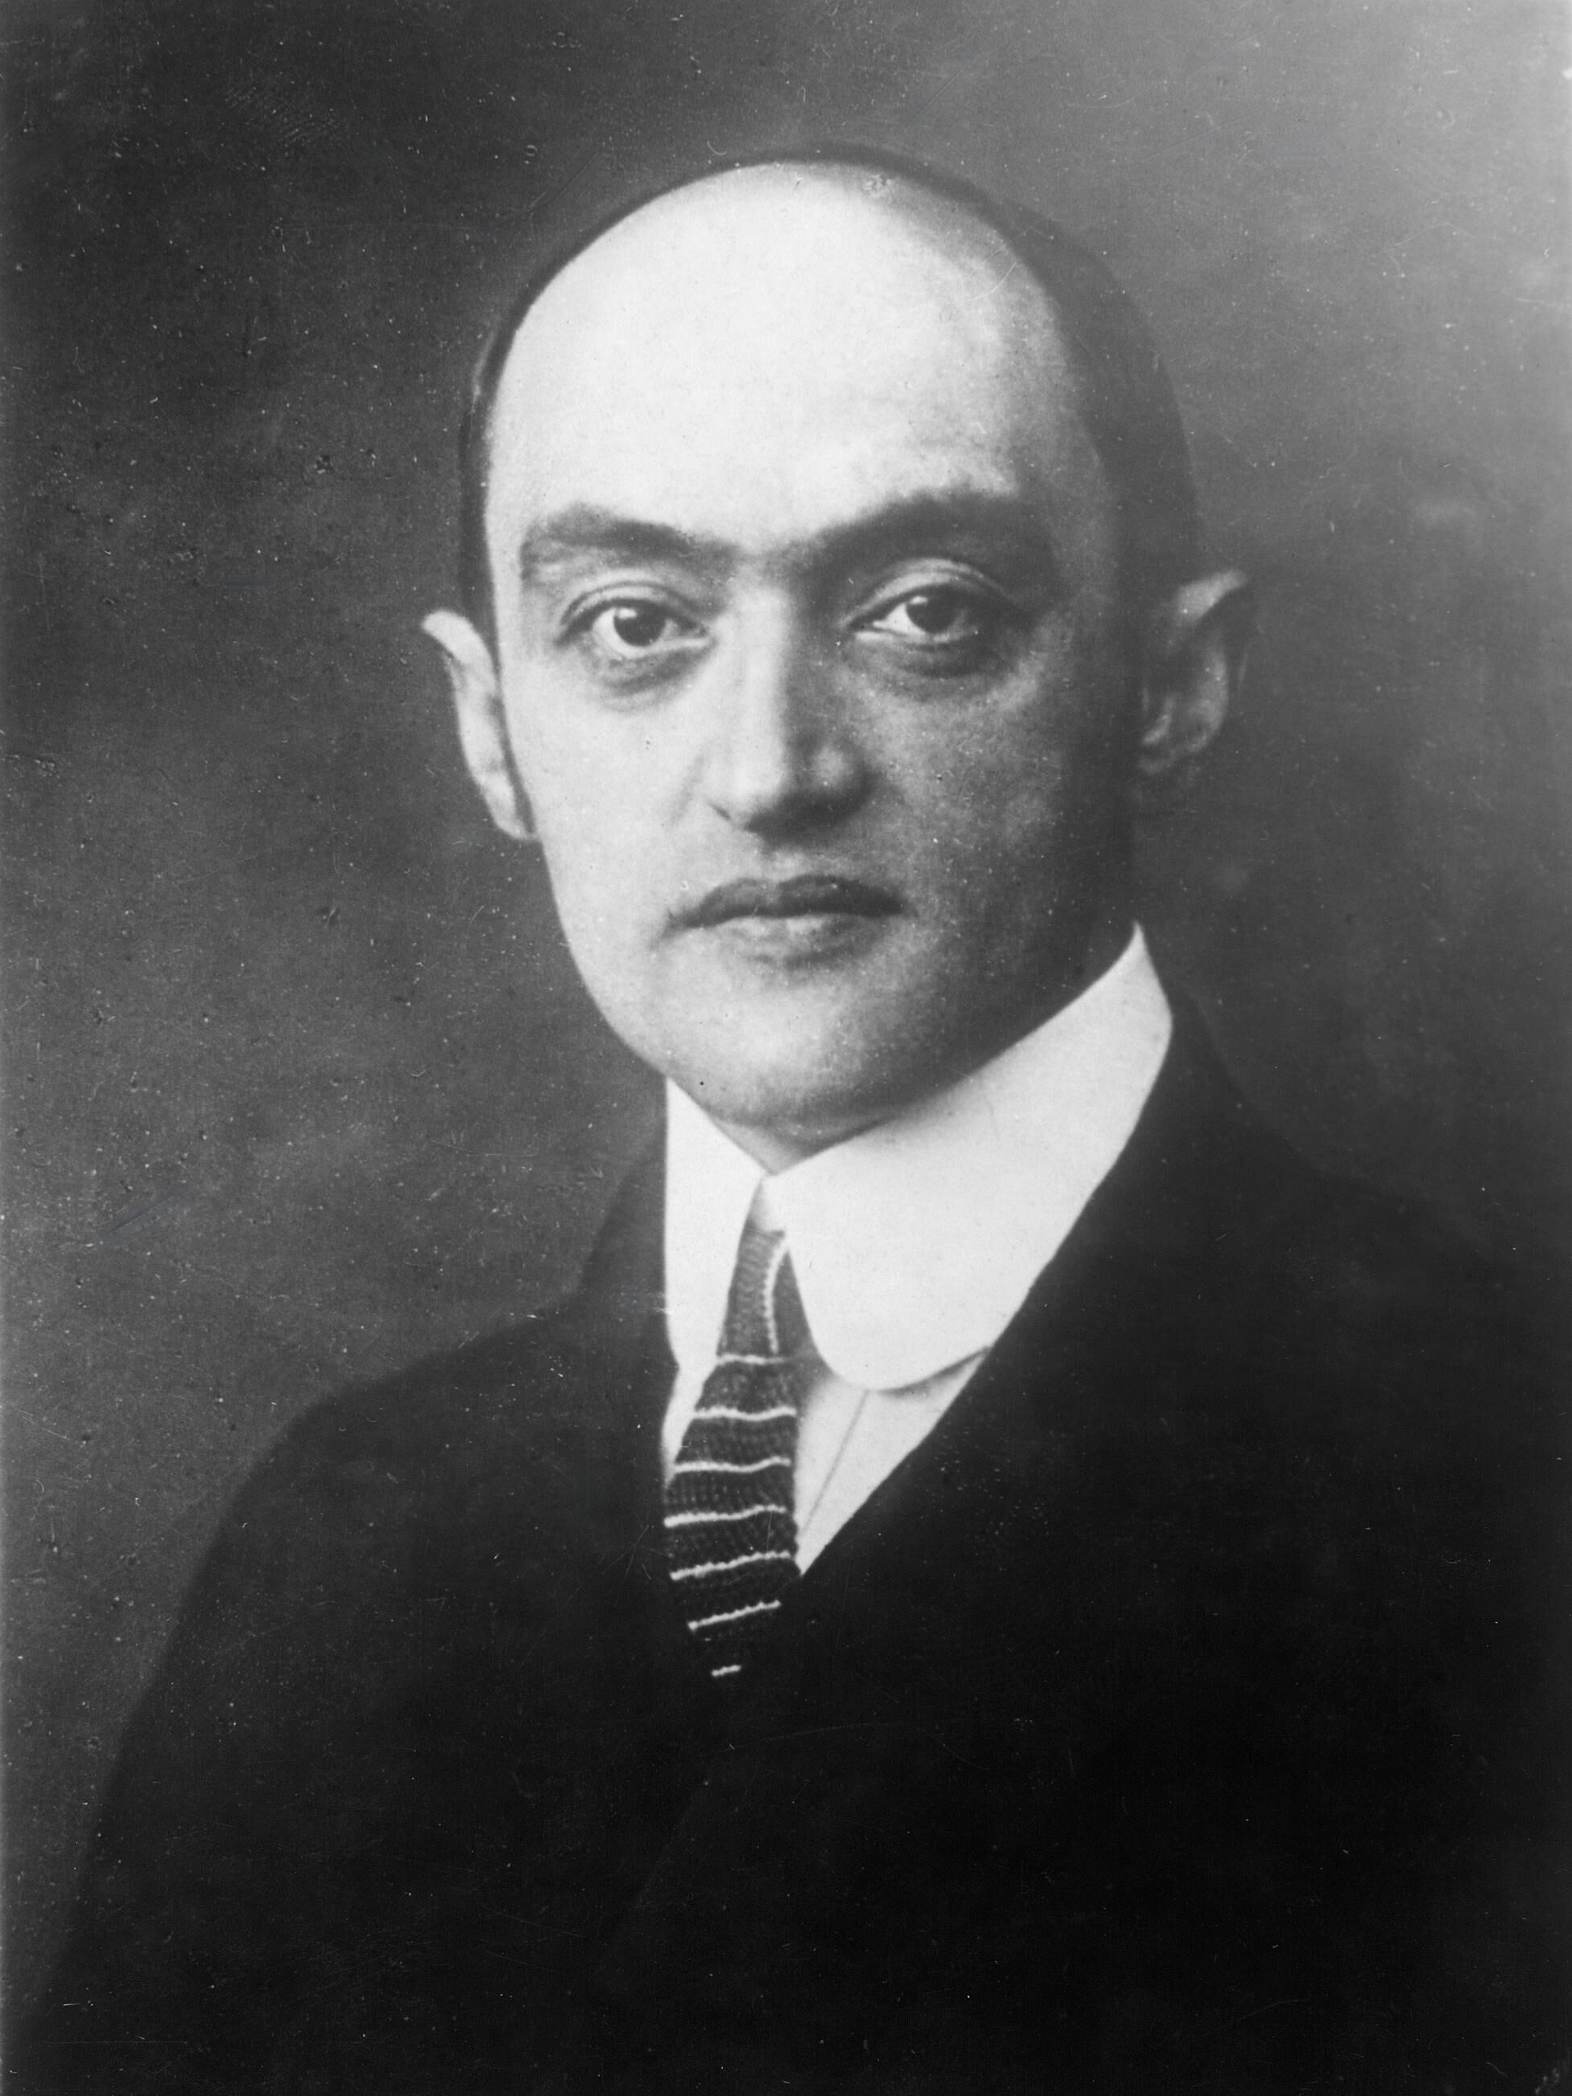
\includegraphics[width=\textwidth]{Joseph_Schumpeter_ekonomialaria.jpg}
                \caption{Schumpeter}
            \end{figure}
        \end{column}
        
        % --- Column 2 ---
        \begin{column}{0.225\textwidth}
            \begin{figure}
                
\includegraphics[width=\textwidth]{Philippe_Aghion.jpg}
                \caption{Aghion}
            \end{figure}
        \end{column}
        
        % --- Column 3 ---
        \begin{column}{0.25\textwidth}
            \begin{figure}
                
\includegraphics[width=\textwidth]{Acemoglu_2016_(3x4_cropped).png}
                \caption{Acemoglu}
            \end{figure}
        \end{column}
    \end{columns}
\end{frame}


\begin{frame}{Ouverture}
\begin{enumerate}
    \item \textbf{Creative Destruction $\rightarrow$ when to innovate:}
    \begin{enumerate}
        \item Creation: An entrepreneur introduces a new technology, obtaining \textit{monopoly} rights.
        \item Destruction: This new technology makes old technologies obsolete.
        \item Winners and Losers: This process creates new wealth and jobs for those involved in the new technology but displaces the firms and workers tied to the old methods.
    \end{enumerate}
    \item \textbf{Directed technological change $\rightarrow$ where to innovate:}
    \begin{enumerate}
        \item Explains why innovation is "directed" toward specific areas. 
        \item Technological progress isn't random; it's an endogenous process (meaning it's determined by forces within the economic system) driven by profit motives.
    \end{enumerate}
     \item \textbf{Growth theory and climate change}:
        \begin{enumerate}
\item Climate change is a threat to economic growth.
\item Green policies can slow down growth.
        \end{enumerate}
\end{enumerate}
\end{frame}



\section{Introduction}

\begin{frame}{}
\centering
\Large Introduction
\end{frame}


\begin{frame}{Introduction - General picture}
    \begin{itemize}
\item Growth is determined by technological change.
\item Technological change is due to firms' decisions about where to invest resources and researchers: innovation is a random process that depends on these elements.
\item Example: dirty and clean innovation. 
\item Firm decisions about innovation and productions can be socially suboptimal due to externalities.
\item Firms invest in polluting technologies rather than clean technologies: the long-term consequences of contamination reduce society's welfare.
    \end{itemize}
\end{frame}

\begin{frame}{Introduction - Questions}
\begin{enumerate}
\item What are the main determinants of firms' decisions when investing in dirty or clean technologies?
\item Will firms without environmental policies switch to clean technologies?
\item Which policies are sufficient to induce firms to switch to clean innovation?
\item What is the social cost of these policies? What is the social cost of doing nothing?
\end{enumerate}
\end{frame}


\begin{frame}{Introduction}
\begin{itemize}
\item Two-sector model of directed technological change: one good is produced using dirty inputs (which cause environmental degradation) and the other using clean inputs.
\item \textbf{Profit-maximizing researchers} drive technological change.
\item Technological change depends on the \textbf{\textit{market size}} and \textbf{\textit{price effects}}.
\item The relative magnitudes of these effects are determined by:
    \begin{enumerate}
\item \textbf{Elasticity of substitution} between clean and dirty goods.
\item \textbf{Relative levels of technological development} in the two sectors.
\item Whether dirty inputs use \textbf{exhaustible resources}.
    \end{enumerate}
\end{itemize}
\end{frame}

\begin{frame}{}
\centering
\Large Model economy 
\end{frame}

\section{Model and results}
\begin{frame}{Model - Utility function}
    \begin{itemize}
\item Households have preferences of the form
        \begin{equation}
            \sum_{t=0}^\infty \frac{1}{(1+\rho)^t} u(C_t, S_t)
        \end{equation}
\item where
        \begin{enumerate}
\item $C_t$ is consumption.
\item $S_t$ is the environmental quality.
\item $\overline{S}$ is the environmental quality in absence of human pollution.
\item $\frac{1}{1+\rho}$ is the discount factor.
        \end{enumerate}
\item $u$ is increasing in $C$ and $S$, twice continuously differentiable, and concave, and satisfies the Inada conditions:
    \begin{equation}
    \lim_{C \rightarrow0}\frac{\partial u(C,S)}{\partial C}= \lim_{S \rightarrow0}\frac{\partial u(C,S)}{\partial S} = \lim_{S \rightarrow 0} u(C,S)= -\infty
    \end{equation}
\item And 
    \begin{equation}
        \frac{\partial u(C,\overline{S})}{\partial S}=0
    \end{equation}
    \end{itemize}
\end{frame}

\begin{frame}{Model - Production Function}
    \begin{itemize}
\item The final ouput is a combination of total clean and dirty inputs:
        \begin{equation}
            Y_t = \Big[ (\textcolor{OliveGreen}{Y_t^c})^{\frac{\varepsilon-1}{\varepsilon}} + (\textcolor{brown}{Y_t^d})^{\frac{\varepsilon-1}{\varepsilon}}\Big]^{\frac{\varepsilon}{\varepsilon-1}}
        \end{equation}
\item Substitutability is given by $\varepsilon \in (0,\infty)$.
\item Dirty and clean aggregate inputs $j\in \{d,c\}$ are aggregations of intermediate machines $x_{ji}$ with $i \in [0,1]$, labor $L_j$, and the productivity of each machine $A_{ji}$:
        \begin{equation}
            \textcolor{OliveGreen}{Y_t^c} = L_{ct}^{1-\alpha} \int_0^1 A_{cit}^{1-\alpha} x^{\alpha}_{cit} di , \quad \textcolor{Brown}{Y_t^d} = R_{t}^{\alpha_2} L_{dt}^{1-\alpha} \int_0^1 A_{dit}^{1-\alpha_1}  x^{\alpha_1}_{dit}di
        \end{equation}
\item $\alpha, \alpha_1, \alpha_2 \in (0,1)$, and $\alpha_1 + \alpha_2 = \alpha$.
    \end{itemize}
\end{frame}


\begin{frame}{Isoquants of Normalized CES Production Functions}
\centering
\begin{tikzpicture}[scale=1.3,>=stealth]
% Axes
\draw[->] (0,0) -- (5,0) node[right] {$Y_d$};
\draw[->] (0,0) -- (0,4) node[above] {$Y_c$};
% σ → ∞ : Perfect substitutes (red line)
% Note: This line does not pass through Y_0 (2, 1.4)
\draw[red, thick] (0,3.2) -- (4.2,0.0) 
node[below right, text=red] at (1,1) {$\sigma \to \infty$};
% σ = 1 : Cobb–Douglas (blue dashed)
% Note: This curve does not pass through Y_0 (2, 1.4)
\draw[blue, dashed, thick, domain=0.6:5, samples=100] 
    plot(\x, {2.4/(\x+0.1) + 0.6}) 
    node[below left, text=blue] at (5,1) {$\sigma=1$};
% σ = 0 : Perfect complements (Corrected L-shape at Y_0)
\draw[black, dashed, thick] (5,1.9) -- (1.6,1.9);
\draw[black, dashed, thick] (1.7,4) -- (1.7,2);
\node[above right] at (3,3) {$\sigma = 0$};
% Reference point Y0

\filldraw[black] (1.7,1.9) circle (2.5pt);
\end{tikzpicture}
\vspace{0.4cm}
\end{frame}


\begin{frame}{Model - Exhaustible resource}
\begin{itemize}
\item The exhaustible resource stock $Q_t$ satisfies the following recurrence equation:
        \begin{equation}
            Q_{t+1} = Q_{t} - R_t
        \end{equation}
\item The extraction cost per unit is given by the non-increasing function
    \begin{equation*}
        c(Q_t)
    \end{equation*}
\item Assume $\alpha_2=0$ so the economy has no exhaustible resource (this assumption will be modified later). 
    \end{itemize}
\end{frame}

\begin{frame}{Model - Market clearing conditions I}
    \begin{itemize}
\item The labor market-clearing condition is
        \begin{equation}
            L_{t}^c + L_{t}^d \leq 1 
        \end{equation}
\item The goods market-clearing condition is given by 
        \begin{equation}
            C_t = Y_t - \psi\bigg( \int_0^1 x_{cit} di + \int_0^1 x_{dit} di \bigg) - c(Q_t)R_t
        \end{equation}
\item $\psi$ is the cost of production of one unit of a machine in terms of final output.
    \end{itemize}
\end{frame}


\begin{frame}{Model - Innovation dynamics I (Directed Technical Research)}
    \begin{itemize}
\item Scientist $i \in [0,1]$ decides whether to do research in sector $j\in \{d,c\}$ and is allocated to one machine $x_{jit}$ with quality $A_{jit}$.
\item The scientist successfully innovate with probability $\eta_j$. 
\item If so, the productivity of the machine $A_{jit}$ increases to $(1+\gamma)A_{jit}$.
\item The scientist earns a one-period patent, becoming an entrepreneur with monopoly rights. 
\item If not, the monopoly rights go randomly to an entrepreneur drawn from the pool of potential entrepreneurs who uses the old technology.
    \end{itemize}
\end{frame}


\begin{frame}{Model - Innovation dynamics II}
    \begin{itemize}
\item Scientists are normalized to $1$ and the market-clearing condition for scientists is
        \begin{equation}
            s_{t}^c + {s}_{t}^d\leq1
        \end{equation}
\item Average productivity in each sector is
        \begin{equation}
            A_{jt}= \int_0^1 A_{jit}di
        \end{equation}
\item In sector $j$ for machine $i$ we have:
        \begin{equation*}
        \mathbb{P}(\text{Machine is updated})=\mathbb{P}(\text{scientist is assigned})\cdot \mathbb{P}(\text{innovation occurs})= \eta_{j}s_{ji}
        \end{equation*}
\item Average innovation then evolves as 
        \begin{equation}
            A_{jt}= (1+\gamma \eta_j s_{jt}) A_{jt-1}
        \end{equation}
    \end{itemize}
\end{frame}


\begin{frame}{Model - Environmental dynamics}
    \begin{itemize}
\item Environmental quality evolves as 
        \begin{equation*}
        S_{t+1} = - \xi Y_{dt} + (1+\delta)S_t
        \end{equation*}
\item With
        \begin{align*}
& - \xi Y_{dt} + (1+\delta)S_t < 0 \Rightarrow S_{t+1}=0\\
& - \xi Y_{dt} + (1+\delta)S_t > \overline{S} \Rightarrow S_{t+1}=\overline{S}
        \end{align*}
\item $\xi$ is the rate of environmental degradation.
\item $\delta$ is the rate of environmental regeneration.
        \end{itemize}
        \begin{definition}[Environmental disaster]
        An environmental disaster occurs if $S_t=0$ for some $t < \infty$. 
        \end{definition}
\end{frame}

\begin{frame}{Model - Big Picture}
    \begin{enumerate}
\item Closed economy with consumers, entrepreneurs, and researchers. 
\item Final output is produced with dirty and clean inputs.
\item Each dirty and clean input is produced using dirty and clean intermediate machines owned by entrepreneurs and corresponding dirty and clean productivities.
\item Researchers allocate their research effort based on expected benefits, which stochastically increases the productivity of the corresponding machine.
\item Production of dirty inputs generates pollution, thereby reducing environmental quality. 
    \end{enumerate}
\end{frame}

\begin{frame}{}
\centering
\Large Environmental Disaster without Exhaustible Resources 
\end{frame}

\begin{frame}{Laissez-Faire Equilibrium}
    \begin{itemize}
        \item \textcolor{Blue}{\textbf{Which is going to be the outcome if there are no environmental policies?}}
        \item \textit{Laissez-Faire} - a decentralized equilibrium.
        \item Simple idea: consumers, entrepreneurs (firms) and scientists are \textbf{maximizing} and market-clearing conditions are \textbf{satisfied}.
        \item We will \textbf{compare this} with the planning problem under policy intervention.
    \end{itemize}
\end{frame}


\begin{frame}{Laissez-Faire Equilibrium}
    \begin{itemize}
        \item Formally...
    \end{itemize}
    \begin{definition}
    An equilibrium is a set of sequences of wages ($w_t$), inputs prices ($p_{jt}$), machines prices ($p_{jit}$), demands for machines ($x_{jit}$), demands for inputs ($Y_{jt}$), labor demands ($L_{jt}$) by input producers $j \in \{c, d\}$, research allocations ($s_{dt}, s_{et}$), and an environment ($S_t$) such that:
\begin{enumerate}
    \item[(i)] ($p_{jit}, x_{jit}$) maximizes profits of the producer of machine $i$ in sector $j$;
    \item[(ii)] $L_{jt}$ maximizes profits of producers of input $j$;
    \item[(iii)] $Y_{jt}$ maximizes the profits of final good producers;
    \item[(iv)] ($s_{dt}, s_{et}$) maximizes the expected profit of a researcher at date $t$;
    \item[(v)] the wage $w_t$ and the prices $p_{jt}$ clear the labor and input markets respectively; and
    \item[(vi)] the evolution of $S_t$ is given by (12).
\end{enumerate}
    \end{definition}
\end{frame}



\begin{frame}{Laissez-Faire Equilibrium - Analysis}
\begin{itemize}
    \item \textcolor{blue}{\textbf{Which are the main determinants of this outcome?}}
    \item Where will researchers choose to innovate?
    \item The expected profit $\Pi_{jt}$ for a scientist engaged in sector $j$ at time $t$ is 
    \begin{equation*}
        \Pi_{jt} = \eta_{jt}(1+\gamma)(1-\alpha) p_{jt}^{\frac{1}{(1-\alpha)}}L_{jt}A_{jt-1}
    \end{equation*}
    \item So, the expected relative benefit between the $clean$ and $dirty$ sectors is
    \begin{equation*}
        \frac{\Pi_{ct} }{\Pi_{dt} } = \frac{\eta_{ct}}{\eta_{dt}}  \times \Bigg(\underbrace{\frac{p_{ct}}{p_{dt}}\Bigg)^{\frac{1}{1-\alpha}} }_{\text{price effect}}\quad \times  \underbrace{\frac{ L_{ct}}{ L_{dt}}}_{\text{market size effect}} \times \quad \underbrace{\frac{ A_{ct-1}}{ A_{dt-1}}}_{\text{direct productivity effect}}      
    \end{equation*}
    \item Effects
    \begin{enumerate}
        \item Price effect: technological change is directed towards the sector with higher selling prices. 
        \item Market size effect: technological change is directed towards the sector with more labor. 
        \item Productivity effect: technological change is directed towards the more productive sector. 
    \end{enumerate}
\end{itemize}
\end{frame}

\begin{frame}{Laissez-Faire equilibrium}
    \begin{itemize}
        \item Denote $\varphi=(1-\alpha)(1-\varepsilon)$.
        \item Relative expected profit can be written as 
        \begin{equation*}
             \frac{\Pi_{ct} }{\Pi_{dt} } =  \frac{\eta_c}{\eta_d} \bigg( \frac{1+\gamma \eta_c s_{ct}}{1+ \gamma \eta_d s_{dt}}\bigg)^{-\varphi-1} \Bigg( \frac{A_{ct-1}}{A_{dt-1}}\Bigg)^{-\varphi}
        \end{equation*}
    \end{itemize}
    \begin{lemma}
        Under \textit{Laissez-Faire}, it is an equilibrium for innovation at  to occur in the clean when:
        \begin{equation*}
            \eta_c A_{c t-1}^{-\varphi} > \eta_d(1+\gamma \eta_c)^{\varphi+1}A_{dt-1}^{-\varphi},
        \end{equation*}
        in the dirty sector only when:
        \begin{equation*}
            \eta_d A_{d t-1}^{-\varphi} > \eta_c(1+\gamma \eta_d)^{\varphi+1}A_{ct-1}^{-\varphi},
        \end{equation*}
\end{lemma}
\end{frame}


\begin{frame}{Laissez-Faire equilibrium}
\begin{block}{Assumption 1}
    At $t=0$ productivity is higher in the dirty sector than in the clean sector.
    $A_{c0} < A_{d0} $
\end{block}
\begin{block}{Proposition 1 - Only dirty growth in the Laissez-Faire}
        Suppose that $\varepsilon >1$ and Assumption 1 holds. Then there exists a unique \textit{Laissez-Faire} equilibrium where innovation always occur in the dirty sector only, and the long-run growth rate of dirty input production is $\gamma \eta _d$
    \end{block}
    \begin{proof}
    Idea $\rightarrow$ Relative expected profits can be expressed only on terms of past productivity and parameters. The condition $A_{c0} < A_{d0}$ will move the technological progress only to the dirty sector.
    \end{proof}
\end{frame}


\begin{frame}{Directed Technical Change}
\begin{block}{Proposition 2 - Environmental disaster under \textit{Laissez-Faire}}
        Suppose that $\varepsilon>1$ and Assumption 1 holds. Then the \textit{Laissez-Faire} equilibrium aways led to an enviromental disaster. 
    \end{block}
    \begin{proof}
        This is a consequence of the unbounded growth of dirty output due to continuous growth of dirty technology.
    \end{proof}

    \begin{itemize}
        \item Introduction of a governmental subsidize $q_t$  such that 
        \begin{equation*}
        \frac{\Pi_{ct} }{\Pi_{dt} } = \frac{(\textcolor{blue}{1+q_t})}{1}\frac{\eta_{ct}}{\eta_{dt}}  \times \bigg(\frac{p_{ct}}{p_{dt}}\bigg)^{\frac{1}{1-\alpha}}  \times  \frac{ L_{ct}}{ L_{dt}} \times \frac{ A_{ct-1}}{ A_{dt-1}} 
    \end{equation*}
    \item Force more profitability of the green sector $\rightarrow$ Increase $A_c$ 
    \end{itemize}
\end{frame}

\begin{frame}{Directed Technical Change}
\begin{block}{Proposition 3 - Environmental disaster and input substitutions}
        When the two inputs are strong substitutes and $\overline{S}$ is sufficiently high, a temporary subsidy to clean research will prevent an environmental disaster. In contrast, when the two inputs are weak substitutes, a temporary subsidy to clean research cannot prevent an environmental disaster.
    \end{block}
\end{frame}

\begin{frame}{}
\centering
\Large Optimal Environmental Policy without Exhaustible Resources 
\end{frame}

\begin{frame}{Socially Optimal Allocation}
    \begin{itemize}
        \item \textcolor{blue}{\textbf{Necessary policies to arrive to social optimal}}
        \item To achieve for social optimal allocation is necessary to correct by 2 externalities:
        \begin{enumerate}
            \item Enviromental externalities due to dirty input producers
            \item The fact that researchers does not internalize the effect of their research in the future.
        \end{enumerate}
        \item Achieved by lump-sum taxes and transfers (subsidies)
        \begin{block}{Definition - Socially optimal Allocation}
        The socially optimal allocation is a dynamic path of final good production $Y_t$, consumption $C_t$, input productions $Y_{jt}$, machine productions $x_{jit}$, labor allocations $L_{jt}$, scientist allocations $s_{jt}$, environmental quality $S_t$, and qualities of machines $A_{jit}$ that maximizes the intertemporal utility of the representative consumer, (1), subject to (4), (5), (7), (8), (9), (11), and (12) (with $R_t \equiv 0$ and $\alpha_2 = 0$). The following proposition is one of our main results.
        \end{block}
    \end{itemize}
\end{frame}


\begin{frame}{Socially Optimal Allocation}
    \begin{block}{Proposition 5 - Social optimal allocation and environmental policies}
    The socially optimal allocation can be implemented using a tax on dirty input (\textit{carbon tax}), a subsidy to clean innovation, and a subsidy for the use of all machines.
    \end{block}
    \begin{itemize}
        \item The optimal tax is given by
        \begin{equation*}
            \tau_t = \frac{\omega_{t+1} \xi}{\lambda_t \hat{p}_{dt}},
        \end{equation*}
        %\begin{equation*}
        %    \tau_t = \frac{\frac{\xi}{\hat{p}_{dt}} \frac{1}{1 + \rho} \sum_{v=t+1}^{\infty} \left( \frac{1 + \delta}{1 + \rho} \right)^{v-(t+1)} I_{S_{t+1},...,S_v < \bar{S}} \partial u(C_v, S_v) / \partial S}{\partial u(C_t, S_t) / \partial C},
        %\end{equation*}
    \item $\omega$ is the costate variable associated with the enviromental quality $S_t$, $\lambda_t$ is the costate variable associated with the consumption good $C_t$, $\hat{p}_{dt}$ if the shadow price of input $j$ (in terms of final ouput)..
    \item The tax is \textcolor{blue}{such that the marginal cost of producing dirty input by one unit must be equal to the resulting marginal benefit in terms of higher enviromental quality in all the next periods}. 
\end{itemize}
\end{frame}

\begin{frame}{Optimal allocation of scientists}
    \begin{itemize}
        \item Scientists will be allocated towards the sector with higher \textbf{social gain} from innovation.
        \item Research is directed towards clean sector whenever
        \begin{equation*}
            \frac{\textcolor{blue}{\eta_c (1 + \gamma \eta_c s_{ct})^{-1}} \sum_{v \ge t} \frac{\partial u(C_v, S_v)}{\partial C} \frac{1}{(1 + \rho)^v} \hat{p}_{cv}^{1/(1-\alpha)} L_{cv} A_{cv}}{ \textcolor{blue}{\eta_d (1 + \gamma \eta_d s_{dt})^{-1}} \sum_{v \ge t} \frac{\partial u(C_v, S_v)}{\partial C} \frac{1}{(1 + \rho)^v} \hat{p}_{dv}^{1/(1-\alpha)} L_{dv} A_{dv}} > 1
        \end{equation*}
        \item In the decentralized case the decision to do research or not in the clear sector was depending mainly on the \textcolor{blue}{blue term}.
        \item For the decentralized case such term represent the individual value of innovation
    \end{itemize}
\end{frame}




\begin{frame}{Structure of Optimal Environmental Regulation}
    \begin{block}{Proposition 6 - Social optimal allocation and environmental policies}
    Suppose that $\varepsilon > 1$ and the discount rate $\rho$ is suffifciently small. Then all innovation switches to the clean sector in finite time, the economy grows asymptocally at rate $\gamma \eta_c$ and the optimal subsidy on profits in the clean sector, $q_t$, is temporary. Moreover, if $\varepsilon > \frac{1}{(1-\alpha)}$ then the optimal carbon tax, $\tau_t$ is temporary.
    \end{block}
\begin{itemize}
\item Result: Taxes and subsidies are enough to modify the direction of innovation.
\item Policy intervention is not permanent: If $\varepsilon > 1$, there exists a time $t \geq 0$ such that $A_{ct} > A_{dt}$, meaning that all research will eventually be directed toward the clean sector.
\item Effectiveness of the policies depends on the substitutability between the two inputs.
\end{itemize}
\end{frame}

\section{Conclusions}

\begin{frame}{}
\centering
\Large Conclusions
\end{frame}

\begin{frame}{Conclusions - non discounted parts}
    \begin{itemize}
        \item The case where $\varepsilon < 1$
        \begin{enumerate}
            \item In this case not policies are useful to mantain economic growth and green transition. The only solution to avoind an enviromental disaster is de-growth.
        \end{enumerate}
        \item Exhaustible resources for the production of dirty inputs
        \begin{enumerate}
            \item In this scenatio the reduction of the resources increases its price, making less attratcie to produce wiht it and making firms switch to clean inputs. 
            \item Is not a real scenario (oil, gas and coal reserves are simple too big)
        \end{enumerate}
        \item Modeling robustness 
        \begin{enumerate}
            \item Pollution affects productivity
            \item Alternative technologies 
            \item Alternative laws of motion of environmental stock
        \end{enumerate}
        \item Cost of delay.
    \end{itemize}
\end{frame}

\begin{frame}{Conclusions}
    \begin{itemize}
        \item Decentralized markets lead to environmental disaster due to externalities in innovation and dirty production.
        \item A socially optimal allocation can be achieved with temporary environmental policies: carbon taxes to reduce polluting production and subsidies to incentivize clean research.
        \item However, the effectiveness of these policies depends on a sufficiently high degree of substitutability between clean and dirty inputs.
        \item If substitutability is too low, an environmental disaster may be unavoidable.
    \end{itemize}
\end{frame}


\section{Comments and discussion}

\begin{frame}{}
\centering
\Large Discussions 
\end{frame}



\begin{frame}{Discussions}
        \textit{All theory depends on assumptions which are not quite true.That is what makes it theory. The art of successful theorizing is to make the inevitable simplifying assumptions in such a way that the final results are not very sensitive. A "crucial" assumption is one on which the conclusions do depend sensitively, and it is important that crucial assumptions be reasonably realistic. When the results of a theory seem to flow specifically from a special crucial assumption, then if the assumption is dubious, the results are suspect}
        \vspace{0.5cm}

        Robert Solow, 1958, \textit{A contribution to the theory of economic growth.}
\end{frame}

\begin{frame}{Discussions - Closed vs. Open Economy}
    $\rightarrow$ Model's current assumption: closed economy. \\
    $\rightarrow$ Now, assume an open economy where domestic policies cannot affect foreign firms.
    \begin{itemize}
        \item Assume $N$ firms are generating a dirty input.
        \item $m \in [0,n)$ domestic firms pay taxes, and $m' \in [n,N]$ foreign firms do not.
        \item The marginal cost for foreign firms ($m'$) will be relatively lower than the marginal cost of domestic firms ($m$), which affects prices $\rightarrow$ The carbon tax has no effect.
        \item With a sufficiently high $\varepsilon$ (elasticity?) between domestic and foreign firms, the local ($m$) firms are displaced from the market, and only the $m'$ polluting firms remain.
        \item Example: imports from developing countries.  
        \item Question: How many $m'$ firms are needed to cause displacement? How quickly does this displacement occur?
    \end{itemize}
\end{frame}

\begin{frame}{Discussions - The $\varepsilon$-Problem}
    $\rightarrow$ Model assumption: one good. \\
    $\rightarrow$ Reality: $\overline{\varepsilon} = \int_0^1 \varepsilon_i di $ \\

\begin{itemize}
    \item When discussing clean and dirty goods, there are many examples where $\varepsilon$ is very low over non-trivial intervals. The meat industry is a good example.
    \item We can express this as:
    \begin{equation*}
        Y_t = \int_0^1 \Big[ (\textcolor{OliveGreen}{Y_{it}^c})^{\frac{\varepsilon_i-1}{\varepsilon_i}} + (\textcolor{brown}{Y_{it}^d})^{\frac{\varepsilon_i-1}{\varepsilon_i}} \Big]^{\frac{\varepsilon_i}{\varepsilon_i-1}} di
    \end{equation*}
    \item For some $j \in [0,1]$, $\varepsilon_j$ is very low.
\end{itemize}
\end{frame}

\begin{frame}{Discussions — The $\varepsilon$ Problem}
\begin{itemize}
    \item This means that at least some of the dirty input $f(Y_{tj}^d, \varepsilon_j)$ will still have to be used.
    \item In the best-case scenario, where all firms have completed the green transition except the one for which elasticity is very low, the environmental situation evolves according to:
    \begin{equation*}
        S_{t+1} = -\xi f(Y_{jt}, \varepsilon_j) + (1+\delta)S_t
    \end{equation*}
    \item The environmental situation continues to worsen even after the green transition (depending on the relative strength of the two terms in the difference equation).
    \item Consumer preferences must shift so that good $j$ is no longer demanded.
\end{itemize}
\end{frame}


\begin{frame}{Discussion – Main Problem}
    \begin{itemize}
        \item Two main points raised by the paper:
        \begin{enumerate}
            \item Different initial levels of production inputs between the dirty and clean sectors.
            \item Competition and entry barriers for clean energy.
        \end{enumerate}
    \end{itemize}
\end{frame}

\begin{frame}{Discussion – Main Problem}
      \begin{itemize}
        \item The paper focuses on an important obstacle to inducing the Green Transition: the stock dimension of dirty physical and knowledge capital.
        \item This is not the first case in history—it is the essence of creative destruction.
        \item However, looking at historical examples, at least one of the following conditions must be satisfied:
        \begin{enumerate}
            \item A shift in preferences.
            \item A disruptive technology.
        \end{enumerate}
    \end{itemize}
\end{frame}

\begin{frame}{Discussion – Institutional Environment}
    \begin{itemize}
        \item \textbf{Corporate environment}
        \begin{enumerate}
            \item Polluting companies have more power $\rightarrow$ they can cannibalize clean (new) companies.
            \item How can this be avoided without harming market mechanisms?
        \end{enumerate}
        \item \textbf{Political environment}
        \begin{enumerate}
            \item The Green Transition is incentivized by environmental policies that have short- to medium-term costs (as shown in the paper).
            \item Why should a policymaker (i.e., a politician) be incentivized to adopt measures that are unpopular among the majority of voters?
            \item Mean-field model of voter/politician behavior.
        \end{enumerate}
    \end{itemize}
\end{frame}

\section{Appendix}

\begin{frame}{Equilibrium profits}
    \begin{enumerate}
        \item Profix maximization of the input producer in sector $j$ at time t.
        \item Find the iso-elastic inverse demand curve for each machine. 
        \item Solve monopolistic machine owner problem. 
        \item Price is a constant markup over marginal cost.
        \item We can find the equilibrium demand for the machine. 
    \end{enumerate}
\end{frame}

\begin{frame}{Equilibrium profits and scientists allocation}
    \begin{enumerate}
        \item Write the expected profits on function of productivity.
        \item Study the expression as function of $1+\varphi$
    \end{enumerate}
\end{frame}

\begin{frame}
    \begin{enumerate}
        \item Find $\lambda_t$, the shadow value of one unit of final good consumption at time t (and also the shadow value of one unit more of consumption).
        \item $\omega$ is the Lagrange mutplier of the environmental constraint dynamics.
        \item Shadow value of enviromental quality at timr $t$ is equal to the marginal utility that it generates in this period plus the shadow value $(1+\delta)$ units of enviromental quality in the next period.
        \item This equation can be solved recursively.
        \item Define the lagrande multplier for the input producitons goods    \item Define the ration $\frac{\lambda_j}{\lambda} = \hat{p}_{jt}$ 
        \item FOCs with respect clean and firty input, for the dirty input one finds that the FOCs has the term $\frac{\omega_{t+1}\xi}{\lambda} \Rightarrow \tau_t = \frac{\omega_{t+1}\xi}{\lambda_t \hat{p}_{dt}}$
    \end{enumerate}
\end{frame}


%------------------------------------------------


%----------------------------------------------------------------------------------------

\end{document}